\documentclass[conference]{IEEEtran}

\usepackage{graphicx} \usepackage{url} \usepackage{hyperref} \usepackage{caption} \usepackage{amsmath}
\usepackage{amssymb} \usepackage{array} \usepackage{listings} \usepackage{color} \usepackage{textcomp}
\usepackage[utf8]{inputenc} \usepackage{natbib} \usepackage{algorithm} \usepackage{tikz}
\usepackage[noend]{algpseudocode}

\usetikzlibrary{shapes.geometric, arrows}

\title{Analysis of Lost-in-Space Star Identification Algorithms}
\author{Glenn Galvizo}

\begin{document}
    \maketitle

    \begin{abstract}
    Star identification is the process of mapping centroids in an image to stars in a catalog.
    Gottlieb's Angle method, Liebe's Dot Angle method, Cole and Crassidis's Spherical and Planar Triangle method,
    Motari's Pyramid method, and Toloei's Composite Pyramid method are modified to fit a general identification process.
    Each method was presented an artificial image, and aspects that were interchangeable among each process were
    normalized.
    In order of end to end running time, each method ranks as follows: Pyramid, Angle, Dot Angle, Planar Triangle,
    Spherical Triangle, Composite Pyramid.
    In order of end to end accuracy, each method ranks as follows: Pyramid, Dot Angle, Spherical Triangle, Angle,
    Planar Triangle, Composite Pyramid.
\end{abstract}
 % Abstract.

    \section{Introduction}\label{sec:introduction}
Ancient mariners could look up at the night sky, point out which stars they were looking at, and navigate across the
globe without the use of maps.
\textit{Constellation queries} refer to approaches to determine which stars are in the sky.
Given an image of the sky, to query for a constellation is to map a select few bright spots in image to stars in
a stellar repository.
\textit{Lost-in-space} refers to an additional constraint on the problem: the absence of knowing where we took
the picture and how we pointed the camera.

%Ancient mariners could look up at the night sky, point out which stars they were looking at, and navigate across the
%globe without the use of maps.
%\textit{Star identification algorithms} refer to computational approaches to determining which stars are in the sky.
%Given an image of the sky, star identification is matching the bright spots in an image to stars in an astronomical
%catalog.
%The device that performs these computations is the star tracker, much like the navigators on the ship.
%\textit{Lost-in-space} refers to an additional constraint on the problem: the absence of knowing where we took
%the picture and how we pointed the camera.

This problem is most prevalent in designing LEO (low Earth orbit) spacecraft.
In order for a craft to point a payload, direct its thrusters, or orient its solar panels, an accurate
\textit{attitude} (another term for orientation) must be known.
There are a few known landmarks in space where some attitude can be extracted (the Earth, the Sun), but this
requires constant direction towards just these objects.
Star trackers do not limit themselves to a single object, rather they use multiple stars within their field of view
to determine their orientation.

%There exist roughly $4{,}500$ stars in the sky visible to the human eye.
%For an image of $n$ stars, the naive approach would be compute $C(4{,}500, n)$ combinations from this collection and
%compare each to some subset of stars found in the image.
%For $n\seq 3$, this requires over $10^{10}$ comparisons.
%As an alternative, we sacrifice storage and precision for speed by searching a separate collection which indexes the
%${\sim}4{,}500$ stars by one or more features.
%When this subset is identified, we determine and return the orientation of the image relative to collection
%of ${\sim}4{,}500$ stars.

This research is motivated by a growing difference in the number of stellar attitude determination methods and
empirical comparison between each of these methods in a more systematic manner for star tracker development.
Interchangeable factors are abstracted away (camera hardware, blob detection, etc\ldots) to focus more on how each
query strategy matches stars in an image to stars in a database.
This paper aims to contribute a hardware independent comparison process, an algorithmic description of several
query strategies, as well as runtime and catalog access analysis of these strategies under various types of noise.
The process of identifying blobs in an image, constructing the image coordinate system, and efficiently querying
static databases are not addressed here.

\subsection{Stellar Based Attitude Determination}\label{subsec:stellarBasedAttitudeDetermination}
%Attitude refers to the translation between how one system describes an object compared to how a different system
%describes the same object.
%
%In the context of spacecraft attitude for star identification, there exist three reference frames: the
%\textit{body frame}, the \textit{sensor frame}, and the \textit{inertial frame}.
%The body frame itself is fixed to the structure of the spacecraft, the sensor frame is fixed to the star tracker,
%and the inertial frame refers to some non-accelerating frame in which stellar objects are recorded.
%All observations from the spacecraft exist in the sensor frame, but can easily be rotated to align with the body frame
%(the sensor itself is fixed to the spacecraft chassis).
%Consequently, the body frame is used interchangeably with the sensor frame.
%To describe the craft itself, an inertial frame is required for finding a practical attitude.
%A star observed in the inertial frame is more predictable than the same star observed in a tumbling spacecraft, aiding
%the usage of the attitude with orientation dependent processes.
%Using all three, the goal of attitude determination becomes finding some method of translation between the inertial
%frame and the body frame.

Let $\kFrame$ describe an inertial reference frame and $\iFrame$ describe a body reference
frame~\cite{wie:spaceVehicleDynamics}.
To find a matrix $A$ that describes the basis vectors of $\kFrame$ in terms of $\iFrame$ but accounts
for the noise of each measurement is known as \textit{Wahba's problem}.
First posed by Gracie Wahba in 1965~\cite{wahba:attitudeEstimationProblem},
Wahba's problem states that finding the optimal $A$ is minimizing the loss function below:
\begin{equation}
    L(A) = \frac{1}{2} \sum_j^n \vv{w_j} \left\| \vv{I_j} - A\vv{K_j} \right\|^2
\end{equation}
where $\vv{w_j}$ represents a non negative weight associated with the noise between the observations $\vv{I_j}$
in the body frame and $\vv{K_j}$ in the inertial frame.
For all instances where Wahba's problem appeared, the \textit{TRIAD method} (short for TRIaxial Attitude Determination)
was used as a closed form solution~\cite{markley:attitudeDeterminationTwoVectors}.

%
%For $n \!>\! 2$, Wahba's problem exists as an optimization problem.
%In the $n\seq2$ case though, the \textit{TRIAD method} (short for TRIaxial Attitude Determination) exists as a
%closed form solution~\cite{markley:attitudeDeterminationTwoVectors}.
%This algorithm starts by constructing two sets of basis vectors: one attached to the body referential (two
%observations in the body frame) $\left[ \vv{t_{1I}} \ \vv{t_{2I}} \ \vv{t_{3I}} \right]$ and another attached to
%the inertial referential (two observations in the inertial frame) $\left[ \vv{t_{2I}} \ \vv{t_{2K}} \ \vv{t_{3K}}
%\right]$~\cite{benet:swisscubeAttitudeDetermination,black:passiveAttitudeDetermination}.
%This is known as the triad frame:
%\begin{alignat}{4}
%    \vv{t_{1I}} &= \frac{\vv{v_1}}{\left| \vv{v_1} \right|} &\vv{t_{2I}} &{}={}&
%    \frac{\vv{u_1}}{\left| \vv{u_1} \right|} \ \ \ \ \ \ \  \\
%    \vv{t_{2I}} &= \frac{\vv{v_1} \times \vv{v_2}}{\left| \vv{v_1} \times \vv{v_2} \right|} \ \ \ \ \ \ \ \
%        &\vv{t_{2K}} &{}={}& \frac{\vv{u_1} \times \vv{u_2}}{\left| \vv{u_1} \times \vv{u_2} \right|} \\
%    \vv{t_{3I}} &= \vv{t_{1I}} \times \vv{t_{2I}} &\vv{t_{3K}} &{}={}& \vv{t_{2I}} \times \vv{t_{2K}}
%\end{alignat}
%Getting from frame $\kFrame$ to $\iFrame$ now simplifies to multiplication of the triad frame base change matrices:
%\begin{equation}
%    A =
%    \begin{bmatrix}
%        \vv{t_{1K}} & \vv{t_{2K}} & \vv{t_{3K}}
%    \end{bmatrix}
%    \begin{bmatrix}
%        \vv{t_{1I}} & \vv{t_{2I}} & \vv{t_{3I}}
%    \end{bmatrix}^T
%\end{equation}

%\begin{subequations}
%Relative to our solar system, the majority of bright stars ($m \!<\! 6.0$, or visible from the Earth with the naked
%eye) do not visibly move.
%Relative to our solar system, the majority of stars visible from Earth with the naked eye do not visibly move.
For simplicity, we make the assumption here that all stars in $\kFrame$ are fixed and exist in an inertial frame
known as the \textit{Earth centered inertial} (ECI) frame.
The star vectors themselves come from astronomical catalogs, recorded as points lying on the celestial
sphere~\cite{tappe:starTrackerDevelopment}.
Two pieces of information are given here: right ascension $\alpha$ (equivalent to latitude on Earth) and
declination $\delta$ (equivalent to longitude).
$\vv{K_j}$ represents a point $\left( \alpha, \delta \right)$ in a 3D spherical frame with a fixed radius for all stars,
projected to 3D Cartesian space.
%    Representing some spherical point $(\alpha, \delta, r)$ in 3D Cartesian space involves the following:
%    \begin{align} \label{eq:sphereToCartesian}
%    x &= r \cos(\delta) \cos(\alpha) \\
%    y &= r \cos(\delta) \sin(\alpha) \\
%    z &= r \sin(\delta)
%    \end{align}
%    where both $\alpha$ and $\delta$ are in degrees, and $r$ represents some constant distance from Earth.
%    $\vv{K_j}$ represents a point obtained from a star catalog that lies in the ECI frame, $r$ units away from Earth.
%\end{subequations}

Let $\vv{I_j}$ represent a 3D point projected from a 2D observation taken by the star tracker.
A basic star tracker is composed of a camera, a computer for determining orientation, and a link back to the main
computer.
After taking the picture, the pixel positions of potential stars in the image are determined.
This involves finding bright blobs in the image, and computing each blob's center of mass to get a point ($x, y$).
Through some 2D to 3D transformation process involving the camera's lens structure, a 3D point is then
obtained~\cite{tappe:starTrackerDevelopment}.
%    To align these stars with the ones in the catalog, the inverse Mercator mapping is used [CITE ME]:
%    \begin{align}
%        x &= k \cos\left( \frac{x}{R}  \right) \cos\left(2 * \arctan\left(\exp\left(\frac{y}{R}\right)\right) -
%            \frac{\pi}{2}\right) \\
%        y &= k \cos\left( \frac{x}{R}  \right) \sin\left(2 * \arctan\left(\exp\left(\frac{y}{R}\right)\right) -
%            \frac{\pi}{2}\right) \\
%        z &= k \sin\left( \frac{x}{R}  \right)
%    \end{align}

The next issue is the focus of this paper: determining which observation from the star tracker frame $\iFrame$
maps to which observation from the star catalog frame $\kFrame$.
Once this correspondence is found, Wahba's problem is solved to obtain $A$ and this is returned to the main computer.
 % Background.

    \section{Star Identification Methods}\label{sec:starIdentificationMethods}

\subsection{Generic Identification Method}\label{subsec:genericIdentificationMethod}
Each identification method is presented with an image $I$ of all the stars in the image reference frame. The goal of
each method is to find some mapping between the \textit{subset} of the image star vectors $b$ and a subset of the
catalog star vectors $r$. This mapping will be denoted as $a$, for alignment. Complete identification of the all stars
in each image is not the focus.

Every algorithm starts with some combination $c$ from all possible $k$ combinations of $|I|$ stars $C_k^{|I|}$, where
$k = $ the size of the image subset that specific identification method uses. A set of stars from the image $b$ is
selected using the current combination $c$.

Using certain features of $b$, a set of catalog star sets $R$ is obtained. $R$ is a list of catalog star candidates as
to which $b$ could map to. Through some filter process, a single set $r$ from $R$ is then selected. The alignment $a$
is then determined between $r$ and $b$. If all of these steps are successful, then this alignment is returned.
Otherwise, a new combination $c$ is selected and the entire process is repeated. This process is detailed
in~\autoref{figure:genericIdentificationMethodFlowchart}.

\begin{figure}
    \centering{
    % Style for process block.
\tikzstyle{process} = [rectangle, text width=3cm, minimum width=3cm, minimum height=1cm,text centered, draw=black,
fill=orange!30]

% Style for terminal block.
\tikzstyle{terminal} = [rectangle, text width=1.7cm, minimum width=1.7cm, minimum height=1.7cm,text centered,
draw=black, fill=red!30]

% Style for decision block.
\tikzstyle{decision} = [diamond, text width=2cm, minimum width=2.5cm, minimum height=2.5cm,text centered, draw=black,
fill=green!30, inner sep=-10pt]

% Style for line.
\tikzstyle{line} = [draw, -latex']

\begin{tikzpicture}[node distance=1.8cm]
    \node[scale=1](getImage)[terminal]{Get Camera Image};
    \node[scale=1](pickQueryStars) [process, left of=getImage, xshift = -1.7cm] {Pick $k$ Image Stars};
    \node[scale=1](searchCatalog)[process, below of=pickQueryStars] {Search Catalog};
    \node[scale=1](confidentInCatalog)[decision, below of=searchCatalog, yshift=-0.5cm] {$|R| > 0$?};
    \node[scale=1](filterCandidates)[process, below of=confidentInCatalog, yshift=-0.5cm] {Filter Candidates};
    \node[scale=1](confidentAfterFilter)[decision, below of=filterCandidates, yshift=-0.5cm] {Confident in $r$?};
    \node[scale=1](findMap)[process, below of=confidentAfterFilter, yshift=-0.5cm]{Identify};
    \node[scale=1](confidentInMap)[decision, below of=findMap, yshift=-0.5cm] {Confident in $a$?};
    \node[scale=1](returnMap)[terminal, right of=confidentInMap, xshift = 1.7cm] {Return Map};

    \draw[->,>=stealth](getImage) -- node[scale=1.3, yshift=-0.3cm]{$I$}(pickQueryStars);
    \draw[->,>=stealth] (pickQueryStars) -- node[scale=1.3, xshift=0.5cm]{$b$}(searchCatalog);
    \draw[->, >=stealth] (searchCatalog) -- node[scale=1.3, xshift=0.5cm, yshift=-0.15cm]{$R$}(confidentInCatalog);
    \draw[->, >=stealth] (confidentInCatalog) -- node[anchor=east, yshift=0.1cm]{Yes}(filterCandidates);
    \draw[->, >=stealth] (filterCandidates) -- node[scale=1.3, xshift=0.5cm, yshift=-0.15cm]{$r$}(confidentAfterFilter);
    \draw[->, >=stealth] (confidentInMap) -- node[xshift=-0.05cm, yshift=0.2cm]{Yes}(returnMap);
    \draw[->, >=stealth] (confidentAfterFilter) -- node[anchor=east, yshift=0.1cm]{Yes} (findMap);
    \draw[->, >=stealth] (findMap) -- node[scale=1.3, xshift=0.5cm, yshift=-0.15cm]{$a$}(confidentInMap);

    \draw[->, >=stealth] (confidentInCatalog.west) -- ++(-1.1cm, 0cm) node[anchor=south, xshift=0.5cm]{No}
    |- (pickQueryStars.west);
    \draw[->, >=stealth] (confidentAfterFilter.west) -- ++(-1.1cm, 0cm) node[anchor=south, xshift=0.5cm]{No}
    |- (pickQueryStars.west);
    \draw[->, >=stealth](confidentInMap.west) -- ++(-1.1cm, 0cm) node[anchor=south, xshift=0.5cm]{No}
    |- (pickQueryStars.west);
\end{tikzpicture}
    \caption{
    Flowchart depicting a general star identification process.
    Given an image $I$, this processes returns an alignment $a$ mapping some subset of the input $b$ to a subset of
    the catalog $r$.
    } \label{figure:genericIdentificationMethodFlowchart}
    }
\end{figure}

% Leaving this out for now. The flowchart should explain the process better.
%\begin{algorithm}[H]
%    \caption{Generic Star Identification Method} \label{algorithm:genericStarIdentification}
%    \begin{algorithmic}[1]
%        \Procedure{Identify}{}
%        \State $I \gets $ all stars from image
%        \For{$c \in r_k^{|I|}$}
%        \State $b \gets \{I(c_1), I(c_2), I(c_3), \dots, I(r_k)\}$
%        \State $R \gets $ catalog star sets, each set of size $=k$
%        \State $r \gets $ a single set from $R$ that matches $b$
%        \State $a \gets $ an alignment between $b$ and $r$
%        \\
%        \If{the steps above are successful}
%        \State \textbf{return} $a$
%        \EndIf
%        \EndFor
%        \EndProcedure
%    \end{algorithmic}
%\end{algorithm}

% Citation: https://digitalcommons.usu.edu/cgi/viewcontent.cgi?article=2723&context=etd AND Gottlieb.
\subsection{Gottlieb's Angle Method}\label{subsec:gottlieb'sAngleMethod}
In 1978, Gottlieb (citation here) developed the Polygon Angular Matching method. Starting with an image $I$, two stars
$b = (b_1, b_2)$ are selected arbitrarily. The corresponding angular separation between each of these stars from a
defined observer is computed, which is denoted as $\theta^{12}$. All possible pairs $(r_i, r_j)$ in the catalog are then
selected such that condition~\eqref{eq:angleRequirement} holds. The set that holds these pairs is denoted as $R$.

\begin{align}
    \label{eq:angleRequirement}
    \begin{split}
        | \theta(r_i, r_j) - \theta^{12} | < 3 \sigma
    \end{split}
\end{align}
$\sigma$ represents the deviation of the uncertainty between the star sensor measurements and the points defined in the
catalog. Assuming the noise follows a Gaussian distribution, it follows that 99.7\% of all true pairs will be within
this range.

If there exists more than one catalog pair after this reduction, then this process is repeated for
$\theta^{13}, \theta^{14}, \dots,$ and so on until a unique pair is found or all possible pairs in the image
have been exhausted. To determine an alignment, a \textit{direct match test} (DMT) is performed.

\begin{algorithm}
    \caption{Angle Identification Method} \label{algorithm:angleIdentification}
    \begin{algorithmic}[1]
        \Procedure{Identify}{}
        \State $I \gets \text{all stars} \text{ from image}$
        \For{$i \gets 1 \text{\textbf{ to }} |I|$}
        \For{$j \gets i + 1 \text{\textbf{ to }} |I| - 1$}
        \State $b \gets (b_i, b_j)$
        \State $R \gets $ catalog pairs that meet~\eqref{eq:angleRequirement} with $b$
        \\
        \If{$|R| = 1$}
        \State $r \gets $ singular pair inside $R$
        \State $a \gets $ \Call{DMT}{$b, r$}
        \State \textbf{return} $a$
        \EndIf
        \EndFor
        \EndFor
        \EndProcedure
    \end{algorithmic}
\end{algorithm}

Tappe (citation here) specifies this DMT method, which extracts an attitude after running this candidate finding step.
Given an image star pair $(b_i, b_j)$ and a catalog star pair $(r_i, r_j)$, an alignment is proposed:
\begin{equation}
    a_1 = (b_i \rightarrow r_i, b_j \rightarrow r_j)
\end{equation}

Wahba's problem (extracting an attitude given vector observations in two coordinate systems) is then solved using the
TRIAD method. This gives a rotation $q_1$ between the image and catalog frames. This process is repeated for the other
possible alignment to obtain a second rotation $q_2$:
\begin{equation}
    a_2 = (b_i \rightarrow r_j, b_j \rightarrow r_i)
\end{equation}

The most likely attitude is determined by predicting which entries in the catalog represent stars in the image using
$q_1$ and $q_2$. The alignment with the most correctly predicted stars is then returned as the resulting attitude.
The general form for this function (accepting an $B$ and $R$ of arbitrary size) is described
in algorithm~\autoref{algorithm:angleHelper}.

\begin{algorithm}
    \caption{Functions for Angle Method} \label{algorithm:angleHelper}
    \begin{algorithmic}[1]
        \Function{DMT}{$b, r$}
        \State $A \gets $ all possible permutations between $b$ and $r$
        \State $M \gets \emptyset$
        \For {$a \in A$}
        \State $q \gets $ \Call{TRIAD}{$a$}
        \State $M \gets M ||$ (stars correctly predicted with $q$)
        \EndFor
        \\
        \State \textbf{return} alignment $a$ associated with \Call{Max}{$M$}
        \EndFunction
    \end{algorithmic}
\end{algorithm}

\subsection{Liebe's Interior Angle Method}\label{subsec:liebe'sInteriorAngleMethod}
In 1995, Liebe (citation here) developed the Liebe Star ID method. Starting with an image $I$, a central star $b_c$ is
selected arbitrarily. The two closest stars in the image to the central star are selected next, denoted as $b_1$ and
$b_2$. Three features are then computed: the angular separation between $b_1$ and $b_c$, the angular separation between
$b_2$ and $b_c$, and the interior angle between $b_1$ and $b_2$ with $b_c$ at the vertex. These are denoted as
$\theta^1, \theta^2,$ and $\phi$ respectively.

The additional constraint that $\theta^1 < \theta^2$ is imposed before proceeding. If this is not true, then stars
$b_1$ and $b_2$ are swapped and this process is repeated. By adding this restriction to the catalog search, a star
alignment procedure (e.g.\ Tappe's direct match test) is no longer required.

All possible \textit{trios} $R$ in the catalog are then selected such that all of
condition~\eqref{eq:interiorAngleRequirement} hold:
\begin{align}
    \label{eq:interiorAngleRequirement}
    \begin{split}
        |\theta(r_i, r_c) - \theta^1| < 3 \sigma_{\theta}
        \\
        |\theta(r_j, r_c) - \theta^2| < 3 \sigma_{\theta}
        \\
        |\phi(r_i, r_j, r_c) - \phi| < 3 \sigma_{\phi}
        \\
        \theta(r_i, r_c) < \theta(r_j, r_c)
    \end{split}
\end{align}

$\sigma_{\theta}$ and $\sigma_{\phi}$ represent the deviation of measurement-catalog uncertainty of angular separations
and interior angular separations respectively. \textit{Note that the $R$ in this procedure is distinct from the $R$ in
the previous Angle method.}

The star trios in $R$ represent potential catalog maps for the image star trio $(b_1, b_2, b_c)$. Liebe's original
method states that this process should be repeated for all stars in the image, meaning that all stars will be the $b_c$
at one point. By the end, each star in the image will have accrued a set of possible catalog matches $P$. The complete
$B \rightarrow R$ map is found by picking the most frequent catalog star appearing in $P$.

To more closely follow the generic star identification flow, $P$ will not be stored and a only one $b_c$ choice will be
needed to acquire a total match. If a confident match is not found by the first $b_c$ star, then the search process
will be repeated until such a match is found. This entire method is described in
algorithm~\autoref{algorithm:interiorAngleIdentification}.

\begin{algorithm}
    \caption{Interior Angle Identification Method} \label{algorithm:interiorAngleIdentification}
    \begin{algorithmic}[1]
        \Procedure{Identify}{}
        \State $I \gets \text{all stars } \text{ from image}$
        \For{$i \gets 1 \text{\textbf{ to }} |I|$}
        \For{$j \gets i + 1 \text{\textbf{ to }} |I| - 1$}
        \For{$k \gets j + 1 \text{\textbf{ to }} |I| - 2$}
        \State $b \gets (b_i, b_j)$
        \State $R \gets $ catalog trios that meet~\eqref{eq:interiorAngleRequirement} with $b$
        \\
        \If{$|R| = 1$}
        \State $(r_i, r_j) \gets $ singular pair inside $R$
        \State $a \gets (b_i \rightarrow r_i, b_j \rightarrow r_j, b_k \rightarrow r_k)$
        \State \textbf{return} $a$
        \EndIf
        \EndFor
        \EndFor
        \EndFor
        \EndProcedure
    \end{algorithmic}
\end{algorithm}

\subsection{Cole and Crassidus's Spherical Triangle Method}\label{subsec:coleAndCrassidus'sSphericalTriangleMethod}
In 2004, Cole and Crassidus (citation here) developed the Spherical Triangle method. Starting with an image $I$, three
stars $b = b_1, b_2, b_3)$ are selected arbitrarily. Treating the trio as a spherical triangle, the spherical area and
moment are computed. This is denoted as $a^{123}$ and $\imath^{123}$ respectively. Similar to Gottlieb's method, star
\textit{trios} $R$ are selected from the catalog such that the all of condition~\eqref{eq:triangleRequirement} hold:
\begin{align}
    \begin{split}
        \label{eq:triangleRequirement}
        | a(r_i, r_j, r_k) - a^{123} | < 3 \sigma_a
        \\
        | \imath(r_i, r_j, r_k) - \imath^{123} | < 3\sigma_{\imath}
    \end{split}
\end{align}
$\sigma_a$ and $\sigma_{\imath}$ represent the deviation of measurement-catalog uncertainty of spherical areas and
moments respectively.

If there exists more than one catalog trio, then a \textit{pivot} is performed. The pivoting process is repeated until
a unique match in $R_{t=1}$ is found, or all possible iterations of the third image star are exhausted. The entire
catalog search procedure is repeated until a unique catalog trio is found, or all trios in the image have been used.
This procedure is described in algorithm~\autoref{algorithm:triangleIdentification}.

\begin{algorithm}
    \caption{Triangle Method Identification} \label{algorithm:triangleIdentification}
    \begin{algorithmic}[1]
        \Procedure{Identify}{}
        \State $I \gets \text{all stars} \text{ from image}$
        \For{$i \gets 1 \text{\textbf{ to }} |I|$}
        \For{$j \gets i + 1 \text{\textbf{ to }} |I| - 1$}
        \For{$k \gets j + 1\text{\textbf{ to }} |I| - 2$}
        \State $R \gets$ \Call{Pivot}{$b_i, b_j, b_k, \emptyset$}
        \If{$R \neq \emptyset$}
        \State \textbf{return} $R$
        \EndIf
        \EndFor
        \EndFor
        \EndFor
        \EndProcedure
    \end{algorithmic}
\end{algorithm}

The pivot procedure starts by setting $R$ to $R_{t=1}$, beginning the pivot with the trio set that was just queried
for. A second set of trios $R_{t=2}$ is retrieved using $\bar{b} = (b_1, b_2, b_4)$, keeping $b_1$ and $b_2$ constant
but changing the third image star. All star trios in $R_{t=1}$ that do not match a trio in $R_{t=2}$ by
\textit{two stars} (a partial match) are removed from $R_{t=1}$. Note that the \Call{Pivot}{$b_i, b_j, b_k, R_1$} call
inside algorithm~\autoref{algorithm:triangleIdentification} defines $R_1 = \emptyset$, which requires a "check" on
lines 2 and 3 of algorithm~\autoref{algorithm:triangleHelper}.

\begin{algorithm}
    \caption{Functions for Triangle Alignment Determination} \label{algorithm:triangleHelper}
    \begin{algorithmic}[1]
        \Function{PartialMatch}{$R_1, R_t$}
        \If {$R_t = \emptyset$} \Comment $t = 1$, no previous set.
        \State \textbf{return} $R_1$
        \EndIf
        \\
        \State $\bar{R_1} \gets \emptyset$
        \ForAll {$v \in R_t$}
        \ForAll {$u \in R_1$}
        \If{two stars in $v$ exist in $u$}
        \State $\bar{R_1} \gets \bar{R_1} || v$
        \State \textbf{break}
        \EndIf
        \EndFor
        \EndFor
        \State \textbf{return} $\bar{R_1}$
        \EndFunction
        \\
        \Function{Pivot}{$b_i, b_j, b_k, R_1$}
        \State $b \gets (b_j, b_j, b_k)$
        \State $R_t \gets $ catalog trios that meet~\eqref{eq:triangleRequirement} with $b$
        \State $R_1 \gets $ \Call{PartialMatch}{$R_t, R_1$}
        \\
        \If{$|R_1| = 1$}
        \State \textbf{return} $R_1$
        \ElsIf{$|R_1| = 0$}
        \State \textbf{return} $\emptyset$
        \Else
        \State $\hat{b_k} \gets \text{an unused star in this pivot}$
        \State \textbf{return} \Call{Pivot}{$b_i, b_j, \hat{b_k}, R_1$}
        \EndIf
        \EndFunction
    \end{algorithmic}
\end{algorithm}

Cole and Crassidus don't specify alignment determination steps, so Tappe's DMT process is used to complete the star
identification process. Given an image star trio $(b_i, b_j, b_k)$ and a catalog star trio $(r_i, r_j, r_k)$, an
alignment is proposed:
\begin{equation}
    a_1 = (s_i \rightarrow r_i, b_j \rightarrow r_j, b_k \rightarrow r_k)
\end{equation}

The TRIAD method only uses two vector observations from each frame, meaning that the $b_k \rightarrow r_k$ map is
disregarded as the first rotation $q_1$ is computed. This process is repeated for all 5 other possible alignments to
get $q_2, q_3, \dots, q_6$.
\begin{description}
    \item [$a_1 = $] $(s_i \rightarrow r_i, b_j \rightarrow r_j, b_k \rightarrow r_k)$
    \item [$a_2 = $] $(s_i \rightarrow r_i, b_j \rightarrow r_k, b_k \rightarrow r_j)$
    \item [$a_3 = $] $(s_i \rightarrow r_j, b_j \rightarrow r_i, b_k \rightarrow r_k)$
    \item [$a_4 = $] $(s_i \rightarrow r_j, b_j \rightarrow r_k, b_k \rightarrow r_i)$
    \item [$a_5 = $] $(s_i \rightarrow r_k, b_j \rightarrow r_i, b_k \rightarrow r_j)$
    \item [$a_6 = $] $(s_i \rightarrow r_k, b_j \rightarrow r_j, b_k \rightarrow r_i)$
\end{description}

For all six attitudes, the $a$ yielding the most correctly predicted stars is returned as the resulting attitude.

\subsection{Cole and Crassidus's Planar Triangle Method}\label{subsec:coleAndCrassidus'sPlanarTriangleMethod}
In 2006, Cole and Crassidus (citation here) developed the Planar Triangle method. This is identical to their Spherical
Triangle method, with the exception that each image trio $b = (b_i, b_j, b_k)$ is represented as a planar triangle
instead of a spherical one.

Computing the spherical moment requires the use of recursion, which could be costly in slower hardware to obtain more
precision. The Planar Triangle method avoids this by computing the planar area and moment instead, which do not require
this recursive step.

% Mortari introduced the use of \textit{search-less} catalog access using the $k$-vector approach, but this will not be
% discussed in this paper.
\subsection{Mortari's Pyramid Star Identification Method}\label{subsec:mortari'sPyramidStarIdentificationMethod}
In 2004, Mortari (citation here) developed the Pyramid method. Starting with an image $I$, three stars
$b = (b_1, b_2, b_3)$ are selected to avoid the persistence of false stars. This is specified in lines 19 to 23 in
algorithm~\autoref{algorithm:pyramidIdentification}. The corresponding angular separation between each distinct
permutation of the three is computed, denoted as $\theta^{12}, \theta^{13}, \theta^{23}$. All possible
\textit{pair sets} $R^{12}, R^{13}, R^{23}$ are selected from the catalog such that
condition~\eqref{eq:angleRequirement} holds for each respective $\theta$. The common stars between each of these $R$
sets is then determined, yielding $T^1, T^2, $ and $T^3$. If there exists a sole element inside each $T$, then a
secondary verification involving guessing a nearby star is performed. Once this verification step is past, an
alignment is then returned. This entire process is described in algorithm~\autoref{algorithm:pyramidIdentification}.

\begin{algorithm}
    \caption{Pyramid Identification Method} \label{algorithm:pyramidIdentification}
    \begin{algorithmic}[1]
        \Function {FindCatalogStars} {$b, I$}
        \State $R^{ij} \gets$ catalog pairs that meet~\eqref{eq:angleRequirement} with ($b_i, b_j$)
        \State $R^{jk} \gets$ catalog pairs that meet~\eqref{eq:angleRequirement} with ($b_i, b_j$)
        \State $R^{ik} \gets$ catalog pairs that meet~\eqref{eq:angleRequirement} with ($b_i, b_k$)
        \\
        \State $T^i \gets $ \Call{Common}{$R^{ij}, R^{ik}, \emptyset$}
        \State $T^j \gets $ \Call{Common}{$R^{ij}, R^{jk}, T^i$}
        \State $T^k \gets $ \Call{Common}{$R^{ik}, R^{jk}, T^i \cap T^j$}
        \\
        \If{$|T^i| = 1 $ \textbf{and} $|T^j| = 1 $ \textbf{and} $|T^k| = 1$}
        \State $r \gets $ singular stars in $T_i, T_j, T_k$
        \If{\Call{Verify}{$r, b, I$} is \textbf{true}}
        \State \textbf{return} $r$
        \Else
        \State \textbf{return} $\emptyset$
        \EndIf
        \EndIf
        \EndFunction
        \\
        \Procedure{Identify}{}
        \State $I \gets \text{all stars } s \text{ from image}$
        \For{$dj \gets 1 \text{\textbf{ to }} |I| - 2$}
        \For{$dk \gets 1 \text{\textbf{ to }} |I| - 1 - dj$}
        \For{$k \gets i \text{\textbf{ to }} |I| - dj - dk$}
        \State $j \gets i + dj$
        \State $k \gets j + dk$
        \\
        \State $b \gets (b_i, b_j, b_k)$
        \State $r \gets$ \Call{FindCatalogStars}{$b, I$}
        \If{$r \neq \emptyset$}
        \State $a \gets (b_i \rightarrow r_i, b_j \rightarrow r_j, b_k \rightarrow r_k)$
        \State \textbf{return} $a$
        \EndIf
        \EndFor
        \EndFor
        \EndFor
        \EndProcedure
    \end{algorithmic}
\end{algorithm}

To find the common stars between two sets of \textit{pairs} $R^{ab}$ and $R^{ac}$, they must be flattened into a single
dimensional set. These new sets are denoted as $\bar{R}^{ab}$ and $\bar{R}^{ac}$ respectively. The function
\Call{Common}{$R^{ab}, R^{ac}, E$} in algorithm~\autoref{algorithm:pyramidHelpers} also specifies an $E$ parameter,
which acts as a "exclusion" set. Once a common star is found (e.g.\ $T^i$), it follows that the next common star to be
found (e.g.\ $T^j$) should not include this previously found star.

The second verification step is denoted as \Call{Verify}{$r, b, I$} in
algorithm~\autoref{algorithm:pyramidHelpers}. This function starts by selecting a nearby star to $b$ in the image $b_e$.
The angular separation between each star in $b$ is computed, generating $\theta^{ie}, \theta^{je}, \theta^{ke}$.
Again, three sets of catalog pairs $R^{ie}, R^{je}, R^{ke}$ are selected such that
condition~\eqref{eq:angleRequirement} holds for each respective $\theta$. If the common star between all $R$ sets
exists near the given $r$ set, then the test past. Otherwise, the test fails.

\begin{algorithm}
    \caption{Functions for Pyramid Alignment Determination} \label{algorithm:pyramidHelpers}
    \begin{algorithmic}[1]
        \Function{Common}{$R^{ab}, R^{ac}, F$}
        \State $\bar{R}^{ab} \gets $ \Call{Flatten}{$R^{ab}$} \Comment set of pairs (2D) to 1D set
        \State $\bar{R}^{ac} \gets $ \Call{Flatten}{$R^{ac}$}
        \State \textbf{return} $(\bar{R}^{ab} \cap \bar{R}^{ac}) - F$
        \EndFunction
        \\
        \Function{Verify}{$r, b, I$}
        \State $b_e \gets $ star in image $I$ not in $b$
        \State $R^{ie} \gets$ catalog pairs that meet~\eqref{eq:angleRequirement} with $(b_i, b_e)$
        \State $R^{je} \gets$ catalog pairs that meet~\eqref{eq:angleRequirement} with $(b_j, b_e)$
        \State $R^{ke} \gets$ catalog pairs that meet~\eqref{eq:angleRequirement} with $(b_k, b_e)$
        \\
        \State $T^e \gets $ \Call{Common}{$R^{je}, R^{ke} \cup R^{ie}, \emptyset$}
        \If{$|T^e| = 1$}
        \State $r_e \gets $ singular star in $T^e$
        \If{$r_e$ is near $r$ in catalog}
        \State \textbf{return true}
        \Else
        \State \textbf{return false}
        \EndIf
        \Else
        \State \textbf{return false}
        \EndIf
        \EndFunction
    \end{algorithmic}
\end{algorithm}

\subsection{Toloei's Composite Pyramid Method}\label{subsec:toloei'sCompositePyramidMethod}
In 2014, Toloei (citation here) developed the Novel Stars ID method, which retains all of the key aspects of Motari's
Pyramid method but uses the features from Cole and Crassidus's Planar Triangle method for the query and reference steps
instead of angles. Starting with an image $I$, three stars $b = (b_1, b_2, b_3)$ are selected arbitrarily. Treating the
trio as a planar triangle, the planar area and moment are computed. This is denoted as $a^{123}$ and $\imath^{123}$
respectively. Similar to the Planar Triangle method, star \textit{trios} $R$ are selected from the catalog such that
condition~\eqref{eq:triangleRequirement} hold.

Unlike the triangle methods, no pivot is performed. This searching process is repeated until a unique $R$ is found. A
similar verification process to the Pyramid method is then performed for all possible alignments\ldots.

\begin{table*}[ht]
    \centering {
    \caption{
    Overview table of the different identification methods. Each method's image features, reduction process,
    and alignment process is displayed.
    } \label{tab:identificationMethodOverview}
    \begin{tabular}{  m{0.22\linewidth} || m{0.21\linewidth} | m{0.21\linewidth} | m{0.24\linewidth} }
        & \textbf{Image Features} & \textbf{Reduction} & \textbf{Alignment} \\
        \hline \hline
        \textbf{Angle} & $\theta^{ij}$ & Require $|R|=1$ & \Call{DMT}{$b, r$} \\ \hline
        \textbf{Interior Angle} & $\theta^{ij}, \theta^{jc}, \phi$ & Require $|R| = 1$ & Restrict $\theta^{ic},
        \theta^{jc}$ at Query Time \\ \hline
        \textbf{Spherical Triangle} & Spherical $a^{ijk}, \imath^{ijk}$ & \Call{Pivot}{$b_i, b_j, b_k, R_1$} &
        \Call{DMT}{$b, r$} \\ \hline
        \textbf{Planar Triangle} & Planar $a^{ijk}, \imath^{ijk}$ & \Call{Pivot}{$b_i, b_j, b_k, R_1$} &
        \Call{DMT}{$b, r$} \\ \hline
        \textbf{Pyramid} & $\theta^{ij}, \theta^{ik}, \theta^{jk}$ & Require $|R| = 1$ &
        \Call{Common}{$R^{ab}, R^{ac}, F$}, \Call{Verify}{$r, b, I$} \\ \hline
        \textbf{Composite Pyramid} & Planar $a^{ijk}, \imath^{ijk}$ & \ldots & \ldots
    \end{tabular}
    }
\end{table*} % Existing Solutions.

    \newcommand{\itmref}[2]{\hyperref[#2]{#1 Variable~\ref*{#2}}}

\section{Methodology}\label{sec:methodology}
The goal of this research was to empirically analyze each identification method, and determine which method most
accurately maps a subset of stars from the catalog to image under the presence of noise.
The general flow of experiments is listed below:
\begin{enumerate}
    \item \textit{Generate} (\autoref{subsec:benchmarkDataGeneration}) an image of stars.
    \item Apply noise to the image.
    \item Give the image to the identification method.
    \item Run the method to a certain step.
    \item Record the output.
    \item Repeat for another image.
\end{enumerate}

Our research goal is directed toward star tracker development, where our input is often very noisy.
Before a raw image can be used in a star identification algorithm it must first go through some process to filter out
extraneous light.
From here, centroid coordinates of an image (i.e.\ stars) are determined in 2D using a center-of-mass approach.
The coordinates are then projected from 2D to the 3D image frame, and then run through the star identification
algorithm~\cite{Survey}.

There are a number of places where error can be introduced here.
What if the filtering removes a star?
What if centroid coordinates are inaccurately determined?
What if the 2D to 3D transformation is inaccurate as well?
In order to quantity star identification error solely, a process must be created to produce an accurate
representation of the 3D image frame.
The exact stars in the image must be known, the date of the image, the field-of-view of the camera, what type of
error exists in the image, \ldots.
As much of the image is supposed to be known, while only varying the star identification algorithm itself.

Unfortunately, obtaining actual images with characterized error is incredibly difficult and not the focus of this
project.
The solution presented here is to remove the reliance on the camera to capture images, and instead
\textit{generate} the images from the catalog used to build the features from.
This parametrizes our hardware (field-of-view, camera direction) and error (Gaussian noise, false stars).

These images are generated using the Hipparcos Input Catalogue v2, an astronomical catalog of recorded stars and their
position relative to Earth.
Once the images were generated, three experiments were performed: one for feature uniqueness, one for reduction
effectiveness, and one for identification performance and accuracy.

All trials were performed on an Intel i7-7700 CPU, 3.60GHz with 16 GB RAM\@.
Each algorithm was implemented in C++14, and compiled with optimization (at \texttt{-O3}).
The exact implementation is available at the following link: \newline
\url{https://github.com/glennga/hoku}.

\subsection{Benchmark Data Generation}\label{subsec:benchmarkDataGeneration}
Benchmark images were generated with the process below:
\begin{enumerate}
    \item Choose a field-of-view, \textit{true attitude}, and an image center.
    \item Select all stars from the catalog that are within the field-of-view of the image center.
    \item Rotate all of these stars from the \textit{catalog frame} to the image frame using the true attitude.
    \item Give the rotated stars, the field-of-view, and the rotated image center to the star identification method.
\end{enumerate}

\begin{subequations}
    \label{eq:catalogToCartesian}
    The catalog here does not refer to the raw Hipparcos Input Catalogue using spherical coordinates, rather a
    modified catalog whose entries exist in a 3D cartesian frame and whose positions are updated to MJD 58119 (January
    2018) from MJD 48319 (March 1991).
    Depicted below is the conversion to ($x, y, z$) points, with $\alpha$ \& $\delta$ in radians,
    $\mu_\alpha$ \& $\mu_\delta$ in radians per year, and $t$ \& $\tau$ (MJD 58119 and time of catalog = MJD 48316
    respectively) in years~\cite{ProperMotion}.
    \begin{align}
        \alpha_t &= \alpha_\tau + \mu_\alpha (\tau - t) \\
        \delta_t &= \delta_\tau + \mu_\delta (\tau - t) \\
        x &= d \times \cos(\delta_t) \cos(\alpha_t) \\
        y &= d \times \cos(\delta_t) \sin(\alpha_t) \\
        z &= d \times \sin(\delta_t)
    \end{align}
\end{subequations}

$d$ in~\autoref{eq:catalogToCartesian} represents the distance from the Earth (an observer) to the star.
For this set of experiments, $d = 1$ to normalize each vector and work entirely on the celestial sphere.
\textit{For simplicity, the \underline{catalog} refers to the set of stars in this Cartesian frame at time = MJD 58119.}

As mentioned before, all catalog stars exist in an inertial frame known as the \textit{catalog frame}.
To generate clean benchmark images, three items must be specified:
\begin{itemize}
    \item An image center in the catalog frame $c_r$.
    \item The field-of-view of the camera $f$.
    \item True attitude to take stars in the catalog frame to the image frame $q_{rb}$.
\end{itemize}

$f$ was chosen to be $20^\circ$ here, but there does exist multiple star trackers with $f < 5^\circ$.
These trackers are often used in conjunction with other sensors (Sun sensors, other star trackers) or recursively
(i.e.\ prior attitude information) to the true attitude $q_{rb}$.
It is assumed here that the only input comes from a single image, and consequently requires a larger $f$.

\begin{figure}
    \centering{
    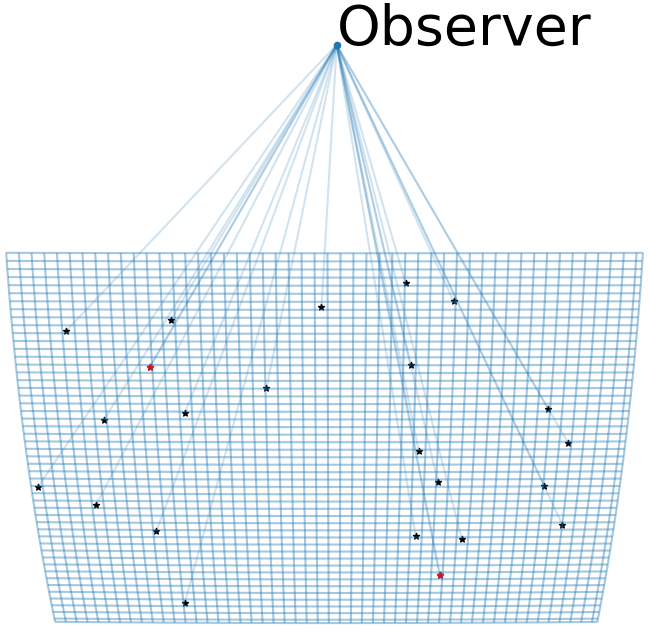
\includegraphics[scale=0.4]{images/benchmark.png}
    \caption{
    Visualization of an image presented to a star identification procedure.
    Stars are represented as vectors whose origin is the observer (i.e.\ Earth), and whose endpoint lies on a section
    of the celestial sphere.
    } \label{figure:benchmarkImageExample}
    }
\end{figure}

All stars from the catalog are selected such that no star exists more than $\frac{f}{2}$ away from the image center.
These stars and the image center are then rotated by $q_{rb}$ to construct the image stars.
The resulting image is presented in~\autoref{figure:benchmarkImageExample}.
What is presented to each identification method are the set of rotated catalog stars, the rotated image center, and
the field of view.

Noise is assumed to exist in two forms here: misrepresentations of the centroid (i.e.\ centroiding error and as
falsely identified sources of light in the image.
Centroiding error is applied to the rotated catalog star set by slightly rotating some star in this set, in some
random direction.
The severity is determined by a Gaussian distribution $N(0, \sigma^2)$.
False stars were added by generating a random vector within $\frac{f}{2}$ of the image center.

\subsection{What are the best hyperparameters for each algorithm?}\label{subsec:hyperparameterSelectionMethods}
This experiment helps determine the optimal hyperparameters (i.e.\ query $\sigma$, overlay $\sigma$) for each
identification method.
Referencing~\autoref{figure:genericIdentificationMethodFlowchart}, different values for this deviation in the
\textit{Search Catalog} step, or "query" step may lead to exclusion of the correct candidates in $R$.
Similarly, differing values for the overlay deviation in the \textit{Identify} step for methods using the
\Call{FPO} call may lead to the wrong map $a$ being selected.

The heuristic used to determine the optimal hyperparameters here was a grid search, iteratively exhausting every
permutation of some set of deviations and measuring the outcome of each trial.
The advantage of this heuristic is that every permutation is tested, but this comes at a cost of time and resources.
For this reason, a smaller number of trials were performed than that of the other experiments when determining
hyperparameters.

To determine the deviation for the query step, a permutation $P_n^{\sigma_n}$ is defined for some integer set $M$,
where:
\begin{equation}
    \label{eq:gridSearchQuery}
    \sigma_n \ \in \ \{ 10^{M_1}, 10^{M_2}, \ldots 10^{M_N} \}
\end{equation}
Each deviation above corresponds to some feature used to query the catalog.
For example, $n = 3$ for the Dot Angle method.
$\sigma_1$ corresponds to $\theta_{ic}$ in the query, $\sigma_2$ corresponds to $\theta_{jc}$, and $\sigma_3$
corresponds to $\phi$.

\begin{subequations}
    \label{eq:defineIdealQuery}
    For each output in~\autoref{eq:querySelectivityMeasures}, a deviation is considered ideal if all queries hit ($I_Q$)
    and have a sole element in the candidate set ($I_S$).
    \begin{align}
        I_Q(i) &=
        \begin{cases}
            1 & \text{if } \frac{Q_i}{N} = 1 \\
            0 & \text{otherwise}
        \end{cases} \\
        I_S(i) &=
        \begin{cases}
            1 & \text{if } \frac{S_i}{N} = 1\\
            0 & \text{otherwise}
        \end{cases}
    \end{align}
\end{subequations}

\begin{subequations}
    \label{eq:idealQuery}
    An ideal region length is the number of indicator variables ($I_Q, I_S$) for some
    consecutive deviation sequence.
    \begin{align}
        \text{Length of ideal } Q \text{ region } &= \sum_{i = 0}^N I_Q(i) \\
        \text{Length of ideal } S \text{ region } &= \sum_{i = 0}^N I_S(i)
    \end{align}
\end{subequations}

% Local Method: https://en.wikipedia.org/wiki/Sensitivity_analysis
\begin{subequations}
    \label{eq:sensitivityQuery}
    For the same outputs in~\autoref{eq:querySelectivityMeasures}, the sensitivity~\cite{SensitivityAnalysis}
    of some critical point $\sigma_c$ can be represented as:
    \begin{align}
        \left\lvert\frac{\partial Q}{\partial \sigma}\right\rvert_{\sigma_{c1}} &= \text{response of } Q \text{ to }
        \sigma \text{ at } \sigma_{c1} \\
        \left\lvert\frac{\partial S}{\partial \sigma}\right\rvert_{\sigma_{c2}} &=
        \text{response of } S \text{ to } \sigma \text{ at } \sigma_{c2}
    \end{align}
\end{subequations}

The more gradual the response is to the candidate set size or probability, the less penalizing an incorrect deviation
choice will be.
The longer that the responses above remain at zero, the less sensitive the hyperparameter selection is for that
specific feature.
The ideal feature set is one that has a long ideal period, and one with low responses to a deviation change.

To determine $\sigma$ for the identification step, the grid search devolves into a linear search.
$\sigma_o$ (overlay) is defined as~\autoref{eq:gridSearchQuery}, for some different set of $M$.

This deviation is used by the \Call{FPO}{} call, a function used by the Angle, Spherical Triangle,
Planar Triangle, and Composite Pyramid methods.
Given that this function operates the same for all identification methods above, this function was tested separately
as a binary classifier.
The sensitivity of this hyperparameter selection was characterized in terms of the resulting recall of the
classification:
\begin{equation}
    \label{eq:sensitivityIdentification}
    \left\lvert\frac{\partial \mathit{TPR}}{\partial \sigma}\right\rvert_{\sigma_o} = \text{response of } \mathit{TPR}
    \text{ at } \sigma_o \\
\end{equation}

Similarly, the longer the response above remains at zero the less sensitive the hyperparameter selection will be for
the \Call{FPO}{} call.

\subsection{Which set of features best distinguish a set of stars?}\label{subsec:querySelectivityMethods}
This experiment helps determine which identification method has the best querying process for catalog candidates $R$.
This is the first filter step, reducing the entire catalog to a subset of combinations.
If the correct stars do not exist here (filter produces false negatives), then the following steps will not be able to
correctly determine a map.
On the other hand if not enough of the catalog is filtered, there is a greater chance of error occurring at later steps.

Differences in catalog querying are specified in each paper (K-Vector, KD Trees, \ldots), but in this set of
experiments all catalog querying uses a B-Tree index.
The only unique portion of each query that remains are what features each method uses to search the catalog.
A general SQL statement to search each image star subset becomes:
\begin{align*}
    \texttt{SELECT } &r_1, r_2, \ldots, r_k \\
    \texttt{FROM } &C \\
    \texttt{WHERE } &(c_{f1} < q_{f1} + 3\sigma_1) \texttt{ AND } (c_{f1} > q_{f1} - 3\sigma_1) \texttt{ AND } \\
    &(c_{f2} < q_{f2} + 3\sigma_2) \texttt{ AND } (c_{f2} > q_{f2} - 3\sigma_2) \texttt{ AND } \\
    &\vdots \\
    &(c_{fn} < q_{fn} + 3\sigma_n) \texttt{ AND } (c_{fn} > q_{fn} - 3\sigma_n)
\end{align*}
\begin{align*}
    k =& \text{ number of stars used in the query.} \\
    c_f =& \text{ catalog feature amongst } r_1, r_2, \ldots, r_k.\\
    q_f =& \text{ image feature amongst an image star subset } b. \\
    n =& \text{ number of features used to query the catalog.} \\
    \sigma_n =& \text{ deviation of Gaussian noise.} \\
    C =& \text{ the catalog.}
\end{align*}

There are five features tested, given that Toloei's Composite Pyramid uses the same features as the Cole and
Crassidus's Planar Triangles method.
\begin{itemize}
    \item Angular separation $\theta^{ij}$ between two stars.
    \item Angular separations $\theta^{ic}, \theta^{jc}$ and dot angle $\phi$ between three stars.
    \item Planar area $a^{ijk}$ and moment $\imath^{ijk}$ between three stars.
    \item Spherical area $a^{ijk}$ and moment $\imath^{ijk}$ between three stars.
    \item Angular separations $\theta^{ij}, \theta^{ik}, \theta^{jk}$ between three stars.
\end{itemize}

\begin{subequations}
    \label{eq:querySelectivityMeasures}
    To quantify the selectivity and accuracy of each feature, we looked at:
    \begin{align}
        \text{Query hit probability } (Q) &= \frac{1}{N} \sum_{i = 0}^N y'(i) \\
        \text{Query selectivity } (S) &= \frac{1}{N} \sum_{i = 0}^{N} \lvert R(i) \rvert
    \end{align}

    Where $N$ is defined as the number of samples and $y'$ is defined as:
    \begin{equation}
        y' =
        \begin{cases}
            1 & \text{if correct star set } \in R \\
            0 & \text{otherwise}
        \end{cases}
    \end{equation}
\end{subequations}

The resulting candidate sets represents one element inside the \textit{set} of $R$ sets.
Repeating this $N$ times would give us the measures in~\autoref{eq:querySelectivityMeasures}.

The running time of each query step $t$ will also be recorded.
This represents the time to retrieve each $R$ set, and will be used to determine the efficiency.
\begin{equation}\label{eq:queryEfficiency}
    \text{Query efficiency } = \frac{1}{|R| \times t}
\end{equation}

An ideal querying processes consists of a query hit probability = 1, a selectivity of 1 candidate set, and a high
efficiency.
The latter is desired as this reduces the amount of work required by the reduction process.

\subsection{What is the best process for reducing catalog candidates?}\label{subsec:candidateReductionMethods}
This experiment helps determine which identification method has the best querying + candidate reduction process.
If a reduction process is too restrictive, then a single match in $R$ will never be found.
If a reduction process is not restrictive enough, then the following steps will rarely determine a correct map.

For a majority of these methods, a reduction process is a matter of repeating the query steps until $\lvert R \rvert=1$
holds true.
For the triangle methods however, their reduction process is the \Call{Pivot}{} method.
The experiment reduces down to $\lvert R \rvert=1$ reduction vs. \Call{Pivot}{} reduction, coupled with each individual
method's query steps.

\begin{subequations}
    \label{eq:reductionAccuracyMeasures}
    To quantify the efficiency of each query + reduction process, we looked at:
    \begin{align}
        \text{Average reduction accuracy} &= \frac{1}{N} \sum_{i = 0}^N y''(i) \\
        \text{Average reduction running time} &= \frac{1}{N} \sum_{i = 0}^N t(i)
    \end{align}

    Where $t$ is defined as the running time to return one $r$ set and $y''$ is defined as:
    \begin{equation}
        y'' = \frac{| r \in \text{original, non-rotated image set}|}{|r|}
    \end{equation}
\end{subequations}

Referencing~\autoref{figure:genericIdentificationMethodFlowchart}, the experiment starts at the \textit{Get Camera
Image} step and executes the identification method to past the \textit{Confident in $r$?} decision block to produce a
single match from the catalog candidate set for some image star subset.
The resulting candidate set represent one element inside the set of $r$ sets.
Repeating this $N$ times would give us the measures in~\autoref{eq:reductionAccuracyMeasures}.

An ideal reduction processes consists of a reduction hit probability = 1 and a short running time compared to the other
reduction processes.
We define the most efficient method as having the highest accuracy to running time ratio.

\subsection{Which method most accurately determines a map?}\label{subsec:identificationMethods}
This experiment helps determine which identification method produces the most accurate catalog to image maps.
An accurate map will reduce an attitude determination problem to Wahba's problem, which can be solved.

\begin{subequations}
    \label{eq:identificationAccuracyMeasures}
    To quantify the efficiency of each identification process (end-to-end), we looked at:
    \begin{align}
        \text{Average identification accuracy} &= \frac{1}{N} \sum_{i = 0}^N y'''(i) \\
        \text{Average identification running time} &= \frac{1}{N} \sum_{i = 0}^N t(i)
    \end{align}

    Where $t$ is defined as the running time to return a complete map and $y'''$ is defined as:
    \begin{equation}
        y''' = \frac{\text{number of correct mappings } b \rightarrow r}{\lvert b \lvert}
    \end{equation}
\end{subequations}

Referencing~\autoref{figure:genericIdentificationMethodFlowchart} again, this experiment runs the identification
method end to end.
Partial accuracy was recorded by counting the number of correct stars against the total amount of stars in a given
map.

An ideal identification method consists of an average identification accuracy = 1 and a short running time compared
to the other identification methods.
We define the most efficient method as having the highest accuracy to running time ratio.
 % Methodology

    \section{Analysis}\label{sec:analysis}

\subsection{Feature Uniqueness}\label{subsec:featureUniquenessAnalysis}
$\epsilon_1, \epsilon_2, \ldots \epsilon_n$ are hyperparameters that must be defined prior to executing the algorithm.
Recall that every $\epsilon$ term defines how selective each query is.
The heuristic used to determine each term was a grid search, where:
\begin{equation}
    \label{eq:gridSearchEpsilon}
    \epsilon_n \ \in \ \{1.0e^{-1}, 1.0e^{-2}, \ldots 1.0e^{-14}\}
\end{equation}
Each experiment was performed $14n$ times , and the largest $\epsilon$ that produced the most query hits are displayed
below.
These were used for all experiments in the results presented here and in the following sections.
\begin{align*}
    \text{Angle / Pyramid}&: \sigma_\theta &= 1.0 \times 10^{-6}\\
    \text{Dot Angle}&: \sigma_{\theta_{ic}} &= 1.0 \times 10^{-4}\\
    \text{Dot Angle}&: \sigma_{\theta_{jc}} &= 1.0 \times 10^{-4}\\
    \text{Dot Angle}&: \sigma_\phi &= 1.0 \times 10^{-4} \\
    \text{Spherical Triangle}&: \sigma_a &= 1.0 \times 10^{-4}\\
    \text{Spherical Triangle}&: \sigma_\imath &= 1.0 \times 10^{-4}\\
    \text{Planar Triangle / Composite}&: \sigma_a &= 1.0 \times 10^{-4} \\
    \text{Planar Triangle / Composite}&: \sigma_\imath &= 1.0 \times 10^{-4}\\
\end{align*}

What is plotted in PUTGRAPHHERE depicts

\subsection{Candidate Reduction}\label{subsec:candidateReductionAnalysis}


\subsection{Alignment Determination}\label{subsec:alignmentDeterminationAnalysis}
In addition to the $\epsilon_n$ parameters used in the previous experiments, a parameter $\sigma_o$ must be defined
prior to executing the \Call{DMT}{} method.
This method is used by the Angle, Spherical Triangle, Planar Triangle, and Composite Pyramid methods.
The heuristic used to determine this value was a linear search, where:
\begin{equation}
    \label{eq:gridSearchSigma}
    \sigma_o \ \in \ \{1.0e^{-1}, 1.0e^{-2}, \ldots 1.0e^{-10}\}
\end{equation}
Each experiment was performed 10 times, and the largest $\sigma_o$ that identification the most stars correctly on
average are displayed below.
These were used for the experiment presented here.
\begin{align*}
    \text{Angle}&: \sigma_o &= 1.0 \times 10^{-4}\\
    \text{Spherical Triangle}&: \sigma_o &= 1.0 \times 10^{-4}\\
    \text{Planar Triangle}&: \sigma_o &= 1.0 \times 10^{-4}\\
    \text{Composite Pyramid}&: \sigma_o &= 1.0 \times 10^{-4}\\
\end{align*}
 % Evaluation.

    \section{Conclusion}\label{sec:conclusion}
Attitude determination is a vital part of all spacecraft missions.
Previously, devices such as magnetometers and Sun sensors would give one observation each in both the body and inertial
frames.
The advantage of star trackers is the presentation of multiple observations with just one device.
Star identification is the process associated that maps observations found in the body frame (i.e.\ the image) to the
inertial frame (i.e.\ the catalog).

Gottlieb's Angle method, Liebe's Dot Angle method, Motari's Pyramid method, Cole and Crassidis's Spherical and
Planar Triangle method, and Toloei's Composite Pyramid method were adjusted to fit a general identification flow
and were analyzed in terms of their query, reduction, and identification steps.
Portions that were interchangeable amongst all methods such as database access and centroid determination were
normalized or removed to focus on the star identification aspect itself.

In all experiments, the Pyramid method ranked first (or close to first) in running time and fairly high in accuracy.
The average short running time is a result of a relatively fast query step, and its accuracy can be attributed to the
verification procedure at identification time.
The Pyramid method is the least sensitive to hyperparameter changes in terms of query size response and accuracy
response.
This method produced the lowest number of catalog candidate sets for a given query, and is the most tolerant of
both Gaussian noise and false stars.

The Angle method had the fastest query step, which stems from the small catalog ($\sim$35 times smaller than
the next larger catalogs, the triangle catalogs).
There were a few instances where the accuracy of the Angle method was greater than the Pyramid method, but this came
at the cost of runtime.
The results produced by the query step heavily impacted the reduction and identification runtime.
For the no noise end-to-end case, this method was a factor of MP200 times slower than the next slowest method (Dot
Angle method).

The Dot Angle method is the most sensitive to hyperparameter changes, but had a larger ideal region than the other
methods.
The catalog for this method was $\sim$105 times larger than the Angle method, and consequently had the longest query
step.
This method handles Gaussian noise the best of all other methods, being the second fastest to identify an image and
being first in how accurate the result is.
In terms of false stars, this method ranks last in accuracy.

The accuracy of the Spherical and Planar Triangle methods rank in between for both Gaussian noise and false stars.
The differences between the spherical and planar triangle features are minuscule compared to the algorithms
encapsulating the features themselves.
These methods produced the smallest amount of candidates on average, which was useful in mitigating the highest
theoretical upper bound for catalog accesses.
Unfortunately, these methods were not the fastest nor were they the most accurate.

The Composite Pyramid method, a composite of the Planar Triangle method's features and the Pyramid method's processes,
ranks last in accuracy and average runtime for images with Gaussian noise 2nd in accuracy for images with just
false stars.
Combining the two methods also means combining the filters associated with each, and the results show inconsistent
runtime due to failing at different stages of the algorithm.
Instead of getting the best of both worlds here, the Composite Pyramid method inherits the worst portions of the two.

Overall, the Pyramid method handles both Gaussian noise and false stars the best in a reasonable amount of time.
If one is working with a small field-of-view with limited stars to choose from and Gaussian noise, the Dot Angle
method works best for using one less star than the Pyramid method.
If speed is not a factor but the field-of-view problem still persists, the Angle method should suffice. % Conclusion.

    \nocite{*} % References.
    \bibliographystyle{unsrt}
    \bibliography{references}
\end{document}
